\section{Algoritmos Genéticos}\label{sec:GenericAlgorithms}

Algoritmos são, segundo o dicionário, processos de cálculo. Os Algoritmos Genéticos (Holland, 1975) não fogem à regra. São procedimentos de procura baseados na mecânica da seleção natural e da genética e bons a navegar em grandes quantidades de dados, procurando por soluções que de outra forma não seria possível descobrir (graças à geração de variantes), encontrando uma solução boa e robusta, segundo uma certa medida de desempenho (fitness criteria).

Este tipo de algoritmos, um tipo de algoritmos evolutivos/ algoritmos de aprendizagem, foram inicialmente desenvolvidos com o objetivo de explicar os processos adaptativos dos sistemas naturais e, com isto, desenhar sistemas artificiais de software que conservassem os mecanismos mais importantes dos sistemas naturais. São, por isso, ideais para problemas de otimização, onde se conhece o objetivo e onde os sistemas de aprendizagem necessitam de medidas de desempenho, sendo normalmente utilizados em problemas de natureza combinatória onde a procura de soluções exige grandes esforços computacionais (6).

Apresentam uma estratégia de pesquisa paralela e estruturada, contudo aleatória, cumprindo o principio básico da seleção natural, descrito por Darwin: “Quanto melhor um indivíduo se adaptar ao seu meio ambiente, maior será sua chance de sobreviver e gerar descendentes.”, ou seja, à medida que o algoritmo itera os pontos a reforçar são aqueles que tem os melhores valores. Apesar de aleatórios, os pontos de pesquisa são direcionados já que exploram informações históricas para encontrar novos pontos de pesquisa partindo daqueles que tiveram melhores desempenhos na iteração anterior, também chamada de geração anterior.

Um Algoritmo Genético (GA) é assim constituído por quatro componentes principais:

\begin{enumerate}

\item A \textbf{Função Objetivo}, o objeto de otimização podendo se aplicar a problemas de otimização, a um conjunto de testes para identificar os indivíduos mais aptos ou até mesmo num problema onde apenas conhecemos o formato das entradas e o valor a otimizar não sendo assim necessário para o algoritmo saber como funciona a função objetivo, sendo apenas necessária ter a função disponível para aplicar aos indivíduos e comparar os resultados. 
\item Os \textbf{Indivíduos}, à semelhança da natureza, o portador do código genético que nada mais é do que uma representação do espaço a pesquisar. São também chamados de cromossomas.
\item A \textbf{Seleção} é uma das partes cruciais do algoritmo. Na maioria dos casos os indivíduos são ordenados de acordo com a função objetivo e é lhes atribuído uma probabilidade que resulta da adequação do individuo em comparação com a população onde se encontra. A escolha é depois feita, aleatoriamente, tendo em conta essas probabilidades de forma a que se escolha os melhor adaptados, não deixando de parte a diversidade da população. Contudo, em outros casos, podem-se aplicar outros métodos de seleção como a seleção por torneio, por classificação ou por ranking.
\item A \textbf{Reprodução} é, geralmente, dividida em três fases. O acasalamento onde são escolhidos dois indivíduos para se reproduzirem gerando dois novos indivíduos. A recombinação, onde os descendentes recebem a parte do código genético do “pai” e da “mãe”. Esta recombinação garante que os indivíduos recebem as informações os permitem ser ainda mais aptos ao meio onde estão inseridos. Por último, a mutação que tem como objetivo maior variabilidade genética e impede que a pesquisa fique estagnada num mínimo local.
\end{enumerate}

\begin{figure}[H]
    \centering
    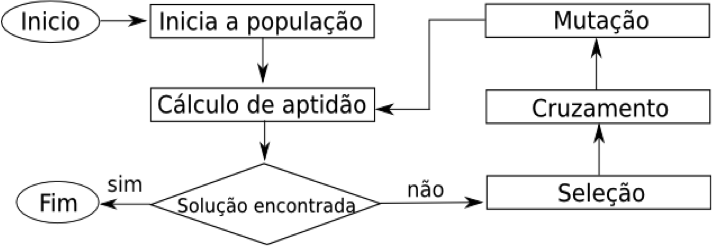
\includegraphics[scale=0.3]{img/ag1.png}
    \caption{Exemplo do processo de um algoritmo genético}
    \label{fig:Processo De Um Algortimo Genetico}
\end{figure}

Em cada geração, são aplicados os princípios de seleção e reprodução a uma população de candidatos. O número de indivíduos desta população varia consoante dois fatores: a complexidade do problema a resolver e os recursos de hardware disponíveis. É através da seleção que se determina quais serão os indivíduos da população que mais facilmente se conseguirão reproduzir, gerando assim os descendentes, com uma probabilidade igual ao seu índice de aptidão (quanto maior o seu índice de aptidão, maiores as chances de se reproduzir). 

Estes algoritmos diferem dos algoritmos genéricos em quatro aspetos (3):
\begin{enumerate}
\item Os Algoritmos Genéticos funcionam com uma representação do conjunto de parâmetros e não com os próprios parâmetros.
\item Os Algoritmos Genéticos funcionam com uma população e não com apenas um ponto.
\item Os Algoritmos Genéticos utilizam informações de recompensa (função objetivo) e não derivadas ou outro conhecimento auxiliar.
\item Os Algoritmos Genéticos utilizam regras de transição probabilísticas e não determinísticas.
\end{enumerate}

Nos sistemas de aprendizagem tenta-se criar soluções para um dado problema partindo de dados ou exemplos (9) de duas maneiras: ou construindo a solução a partir dos dados disponíveis ou procurando uma solução no conjunto de dados. Este segundo método de aprendizagem pode ser feito recorrendo aos algoritmos mais convencionais, contudo o tempo e os recursos necessários para tal tornam-no em algo praticamente impossível, levando a que os Algoritmos Genéticos sejam uma forma mais efetiva de o fazer já que: 
\begin{enumerate}
\item usam conjuntos de dados discretos;
\item são algoritmos de reforço, ou seja, a certeza dos resultados pode ser medida (9) e evolve em gerações;
\item em alguns casos a melhor solução de um problema são várias soluções. 
\end{enumerate}

Por exemplo, num jogo de xadrez os Algoritmos Genéticos nunca seriam usados para ensinar a máquina a jogar mas sim para procurar o melhor movimento a cada jogada

Para quase todos os problemas de computação, é provável que facilmente encontraremos um algoritmo sequencial que o resolve melhor que qualquer Algoritmo Genético. No entanto, esse não é esse o seu intuito. Os AGs são usados quando o nosso problema é uma série de problemas ou quando os seus parâmetros a analisar são muito diferentes (8).

Por exemplo, a programação da função “andar” na robótica é algo extremamente complicado e que pelos algoritmos sequenciais certamente iria falhar. Mesmo, em caso de sucesso, a solução nunca se poderia aplicar a outro robot porque as suas características ou as do meio poderiam mudar. É então mais vantajoso usar Algoritmos Genéticos para “aprender o robot a aprender a andar” em vez de “aprender o robot a andar” e aí encontramos a grande diferença deste tipo de algoritmos (8).